\documentclass[conference]{IEEEtran}
\IEEEoverridecommandlockouts
% The preceding line is only needed to identify funding in the first footnote. If that is unneeded, please comment it out.
\usepackage{cite}
\usepackage{amsmath,amssymb,amsfonts}
\usepackage{algorithmic}
\usepackage{graphicx}
\usepackage{textcomp}
\usepackage{xcolor}
\usepackage[utf8]{inputenc}
\usepackage{textcomp}
\usepackage{caption}

\def\BibTeX{{\rm B\kern-.05em{\sc i\kern-.025em b}\kern-.08em
    T\kern-.1667em\lower.7ex\hbox{E}\kern-.125emX}}
\begin{document}

\title{Design, Simulation and Analysis of a 5 GHz SRR Notch Filter Using Ansys HFSS}

\author{\IEEEauthorblockN{Basireddy Khyathi Sri}
\IEEEauthorblockA{\textit{Department of ECE} \\
\textit{IIIT Hyderabad}\\
Gachibowli, India \\
khyathisri.basireddy@students.iiit.ac.in \\
\textbf{Contribution:} Circular SRR design,\\ Quarter wave transformer}
\and
\IEEEauthorblockN{Chamarthy Madhan Sai Krishna}
\IEEEauthorblockA{\textit{Department of ECE} \\
\textit{IIIT Hyderabad}\\
Gachibowli, India \\
chamarthymadhan.k@students.iiit.ac.in\\
\textbf{Contribution:} Literature review, Report, \\ Quarter wave transformer}
\and
\IEEEauthorblockN{Priyanshi Jain}
\IEEEauthorblockA{\textit{Department of ECE} \\
\textit{IIIT Hyderabad}\\
Gachibowli, India \\
priyanshi.jain@research.iiit.ac.in\\
\textbf{Contribution:} --}
\and
% \hspace{2cm}
\IEEEauthorblockN{Sanjana Sheela}
\IEEEauthorblockA{\textit{Department of ECE} \\
\textit{IIIT Hyderabad}\\
Gachibowli, India \\
sanjana.sheela@students.iiit.ac.in\\
\textbf{Contribution:} Literature review, Electric coupling,\\ Square SRR}
\and
\IEEEauthorblockN{Snigdha}
\IEEEauthorblockA{\textit{Department of ECE} \\
\textit{IIIT Hyderabad}\\
Gachibowli, India \\
snigdha.stp@students.iiit.ac.in\\
\textbf{Contribution:} Quarter Wave Transformer,\\ Impedance Matching }
\and
}

\maketitle

\begin{abstract}
This paper presents the design and simulation of a split ring resonator (SRR) based notch filter operating at a resonant frequency of 5 GHz. The design utilizes a microstrip line coupled with an SRR to achieve a band-stop response. The electromagnetic simulation and optimization of the filter are performed using ANSYS HFSS software. The fundamental principles of SRR notch filters are discussed, and the impact of geometrical parameters on the filter's characteristics is analyzed. This work demonstrates the potential of SRRs for creating compact notch filters suitable for various microwave applications, including the suppression of unwanted signals in communication systems.
\end{abstract}

\begin{IEEEkeywords}
Split Ring Resonator (SRR), Notch filter, 5GHz, Ansys HFSS, Simulation, Design, Microstrip Line, Metamaterials, Band-stop filter, Resonant frequency
\end{IEEEkeywords}

\section{Introduction}

\subsection{Theoretical Background of SRR Notch Filters}
The Split Ring Resonator (SRR) is a type of metamaterial structure that exhibits unique electromagnetic properties, particularly at microwave frequencies. The SRR consists of a pair of concentric rings with a gap, which allows for the manipulation of electromagnetic waves. When excited at its resonant frequency, the SRR can create a band-stop response, effectively filtering out specific frequency bands while allowing others to pass through. This property makes SRRs suitable for applications in wireless communication systems, where interference mitigation is crucial.

\subsection{Motivation and Objectives}
\subsubsection{Motivation}
\textit{Problems with Traditional Filters:} 
\begin{itemize}
    \item \textit{Bulky Size:} Traditional filters based on $ \frac{\lambda}{2} $ or $ \frac{\lambda}{4} $ structures are physically large, making miniaturization difficult.
    \item \textit{Lower Selectivity:} Conventional filters may not sharply reject undesired frequencies(Q-factor).
    \item \textit{Poor Planar Integration}: Not all traditional filters are compatible with PCB or planar technologies.
\end{itemize}

\textit{Advantages of SRR-based Filters:}
\begin{itemize}
    \item \textit{Compact Size:} SRRs can be designed to be much smaller than traditional filters, making them suitable for modern compact devices.
    \item \textit{ High Selectivity:} The resonant nature of SRRs allows for sharp frequency rejection, improving filter performance.
    \item \textit{Planar Integration:} SRR structures can be easily integrated into PCB designs, facilitating mass production and cost-effectiveness.
\end{itemize}
\subsubsection{Objectives}
This project focuses on the design and simulation of a \textbf{Split Ring Resonator (SRR)} intended to operate as a \textit{notch filter} with a target resonant frequency of 5~GHz. The goal is to effectively attenuate signals around the resonant frequency while permitting others to pass through. The design requirements are summarized in the below table:

\begin{table}[ht]
\centering
\begin{tabular}{|l|l|}
\hline
\textbf{Parameter} & \textbf{Requirement} \\ \hline
Resonator Type     & Split Ring Resonator (SRR) \\ \hline
Operating Frequency & $ < $ 6 GHz \\ \hline
Resonant Frequency  & 5 GHz \\ \hline
S$_{11}$ (Input Reflection) & $<$ $-5$ dB at resonance \\ \hline
S$_{21}$ (Transmission) &$ >$ $-10$ dB at resonance (Notch filter) \\ \hline
Sensitivity         & $> $ 10\% \\ \hline
Size                & As compact as possible \\ \hline
\end{tabular}
\caption*{Design specifications for the SRR-based notch filter.}
\end{table}

\subsection{Paper Organization}
The next part of the paper is organized as follows: Section II provides a theoretical framework for understanding the electromagnetic principles behind SRRs and their coupling mechanisms. Section III outlines the design methodology, including substrate selection, topology choice, and parametric analysis. Section IV details the simulation methodology using Ansys HFSS, including model creation and parameter sweeps. Section V presents the results and analysis of the simulation, focusing on resonance frequency, quality factor, and S-parameter results. Finally, Section VI concludes the paper with a summary of findings and future work.

\section{Theoretical Framework}

\subsection{Electromagnetic Theory of SRRs}
\section*{Electromagnetic Theory of SRRs}

A Split Ring Resonator (SRR) is a subwavelength metallic ring structure with a split (gap), commonly used in metamaterial and filter designs. Its unique electromagnetic response is fundamentally governed by Maxwell’s equations, as outlined below:

\subsection*{(a) Faraday’s Law of Induction (Maxwell–Faraday Equation)}

Equation:
\[
\nabla \times \mathbf{E} = -\frac{\partial \mathbf{B}}{\partial t}
\]

% Physical Meaning:
% \begin{itemize}
%     \item A time-varying magnetic field ($\mathbf{B}$) induces a circulating electric field ($\mathbf{E}$).
%     \item In an SRR, an alternating magnetic field passing through the ring induces an electromotive force (EMF).
%     \item This EMF drives circulating currents along the metallic ring.
% \end{itemize}

SRR Interpretation:
\begin{itemize}
    \item The induced current represents the inductive behavior of the SRR.
    \item The EMF is proportional to the rate of change of magnetic flux through the ring.
    \item This allows the SRR to strongly interact with magnetic fields near its resonant frequency.
\end{itemize}

\subsection*{(b) Ampère’s Law (with Maxwell’s Correction)}

Equation:
\[
\nabla \times \mathbf{H} = \mathbf{J} + \frac{\partial \mathbf{D}}{\partial t}
\]

% Physical Meaning:
% \begin{itemize}
%     \item Describes the relationship between magnetic field circulation and the total current (conduction + displacement).
%     \item Conduction current ($\mathbf{J}$) flows in the metal; displacement current arises across the gap.
% \end{itemize}

SRR Interpretation:
\begin{itemize}
    \item Conduction current flows along the ring, generating a magnetic field.
    \item Displacement current across the split gap results from time-varying electric fields.
    \item The interaction forms a resonant LC circuit with oscillations at a specific frequency.
\end{itemize}

\subsection*{(c) Gauss’s Law for Magnetism}

Equation:
\[
\nabla \cdot \mathbf{B} = 0
\]

% Physical Meaning:
% \begin{itemize}
%     \item Magnetic field lines are continuous and form closed loops; no magnetic monopoles exist.
% \end{itemize}

SRR Interpretation:
\begin{itemize}
    \item Magnetic flux generated by ring currents forms closed loops inside and outside the SRR.
    \item Ensures effective inductive behavior by tightly coupling the flux to the SRR.
    \item The linked flux is given by: $\Phi = L \cdot I$, where $L$ is inductance.
\end{itemize}

\subsection*{(d) Gauss’s Law for Electricity}

Equation:
\[
\nabla \cdot \mathbf{D} = \rho
\]

% Physical Meaning:
% \begin{itemize}
%     \item Describes how electric displacement field $\mathbf{D}$ is related to free charge density $\rho$.
% \end{itemize}

SRR Interpretation:
\begin{itemize}
    \item At the split, charge accumulates at the edges, forming an electric field across the gap.
    \item This gap acts as a capacitor, with value dependent on gap size, area, and permittivity.
    \item The SRR behaves as an LC circuit, with resonant frequency:
    \[
    f_r = \frac{1}{2\pi\sqrt{LC}}
    \]
\end{itemize}


\subsection{Equivalent Circuit Models}

\textit{Single Ring Circular SRR:} 
\begin{figure}[h]
\centering
    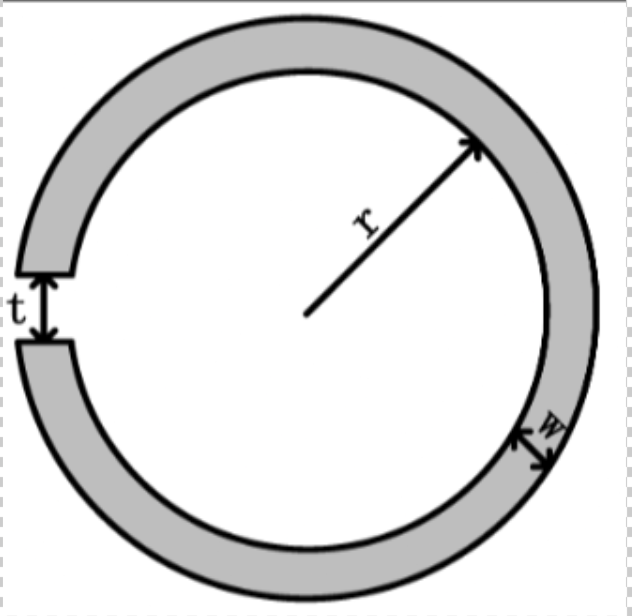
\includegraphics[width=0.2\textwidth]{Images/Single_Ring_SRR.png}
    \caption{Single Ring Circular SRR.}
    % \label{fig:SRR_circuit}
\end{figure}

\begin{figure}[h]
\centering
    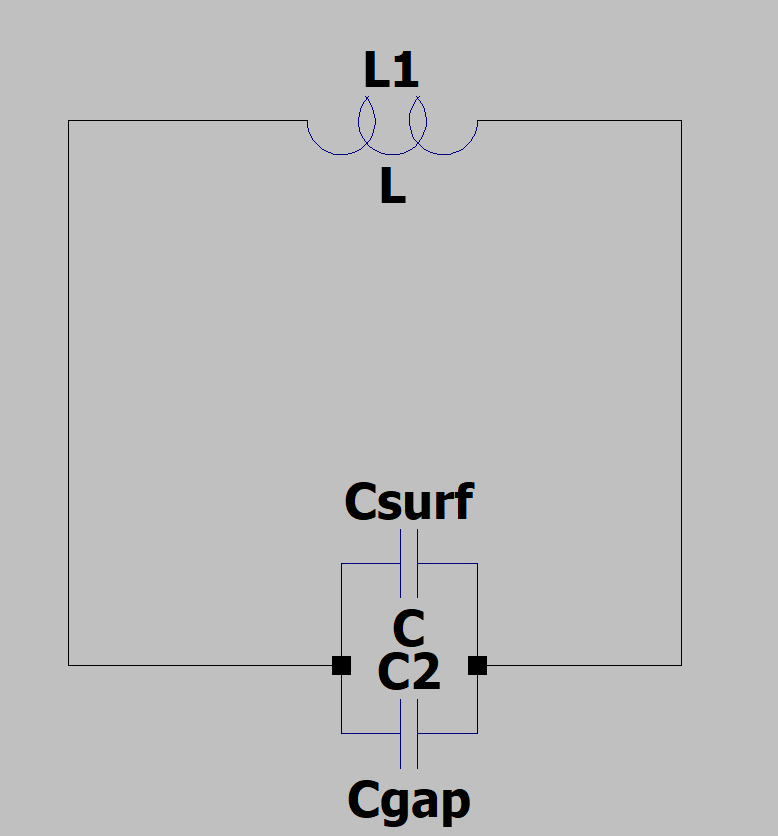
\includegraphics[width=0.2\textwidth]{Images/Single_Circular_Equivalent_model.png}
    \caption{Equivalent circuit model of a Single Ring SRR.}
    % \label{fig:SRR_circuit}
\end{figure}

\begin{equation}
    L = \mu_0 \left( R + \frac{W}{2} \right) \left( \ln\left( \frac{8\left( R + \frac{W}{2} \right)}{h + w} \right) - 0.5 \right)
    \end{equation}
    
    \begin{equation}
    C_{\text{gap}} = \varepsilon_0 \left[ \frac{wh}{t} + \frac{2\pi h}{\ln\left( \frac{2.4h}{w} \right)} \right]
    \end{equation}
    
    \begin{equation}
    C_{\text{total}} = C_{\text{gap}} + C_{\text{surface}}
    \end{equation}
\textit{Double Ring Circular SRR:}
\begin{figure}
\centering
    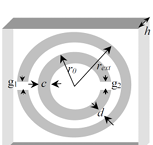
\includegraphics[width=0.2\textwidth]{Images/Double_Ring_SRR.png}
    \caption{Double Ring SRR.}
    % \label{fig:SRR_circuit}
\end{figure}

\begin{figure}
\centering
    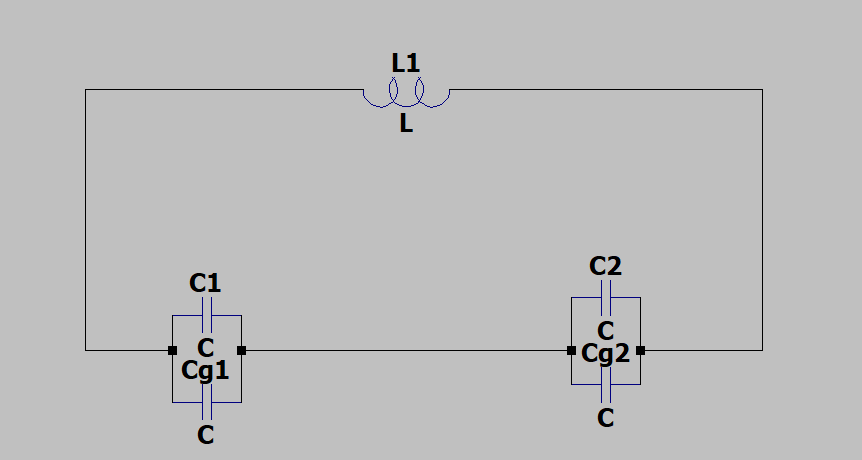
\includegraphics[width=0.3\textwidth]{Images/Double_Circular_Equivalent_modle.png}
    \caption{Equivalent circuit model of a Double Ring SRR.}
    % \label{fig:SRR_circuit}
\end{figure}
\begin{equation}
    f_{0s} = \frac{1}{2\pi \sqrt{L_r C_{eq}}} 
    = \frac{1}{2\pi \sqrt{L_r \left[ \left(2a_{\text{avg}} - \frac{g}{2} \right) C_{\text{pul}} + \frac{\varepsilon_0 c h}{2g} \right] }}
    \end{equation}
    
    \noindent
    where:
    \begin{itemize}
        \item \( f_{0s} \) is the resonance frequency
        \item \( L_r \) is the ring inductance
        \item \( C_{eq} \) is the equivalent capacitance (sum of metal-ring and gap capacitance)
        \item \( a_{\text{avg}} \) is the average radius
        \item \( g \) is the gap
        \item \( c \) is the width of the metal trace
        \item \( h \) is the substrate height
        \item \( \varepsilon_0 = \frac{1}{36\pi} \times 10^{-9} \, \text{F/m} \) (free space permittivity)
    \end{itemize}
    
    \begin{equation}
    C_{\text{pul}} = \frac{\sqrt{\varepsilon_e}}{c_0 Z_0}
    \end{equation}
    
    \noindent
    where:
    \begin{itemize}
        \item \( \varepsilon_e \) is the effective dielectric constant
        \item \( c_0 = 3 \times 10^8 \, \text{m/s} \) is the speed of light in vacuum
        \item \( Z_0 \) is the characteristic impedance of the transmission medium
    \end{itemize}
    
    \begin{equation}
    L_T = 0.00508 \, l \left( 2.303 \log_{10}\left( \frac{4l}{d} \right) - \theta \right)
    \end{equation}
    
    \noindent
    where:
    \begin{itemize}
        \item \( l \) is the conductor length
        \item \( d \) is the diameter
        \item \( \theta \) is a geometry correction constant
    \end{itemize}

\textit{Double Ring SRR with Transmission Line:}
\begin{figure}
\centering
    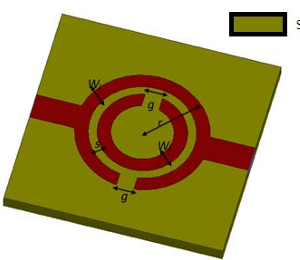
\includegraphics[width=0.25\textwidth]{Images/Double_Ring_SRR_Transmission_line.png}
    \caption{Double Ring SRR with Transmission Line.}
    % \label{fig:SRR_circuit}
\end{figure}

\begin{figure}
\centering
    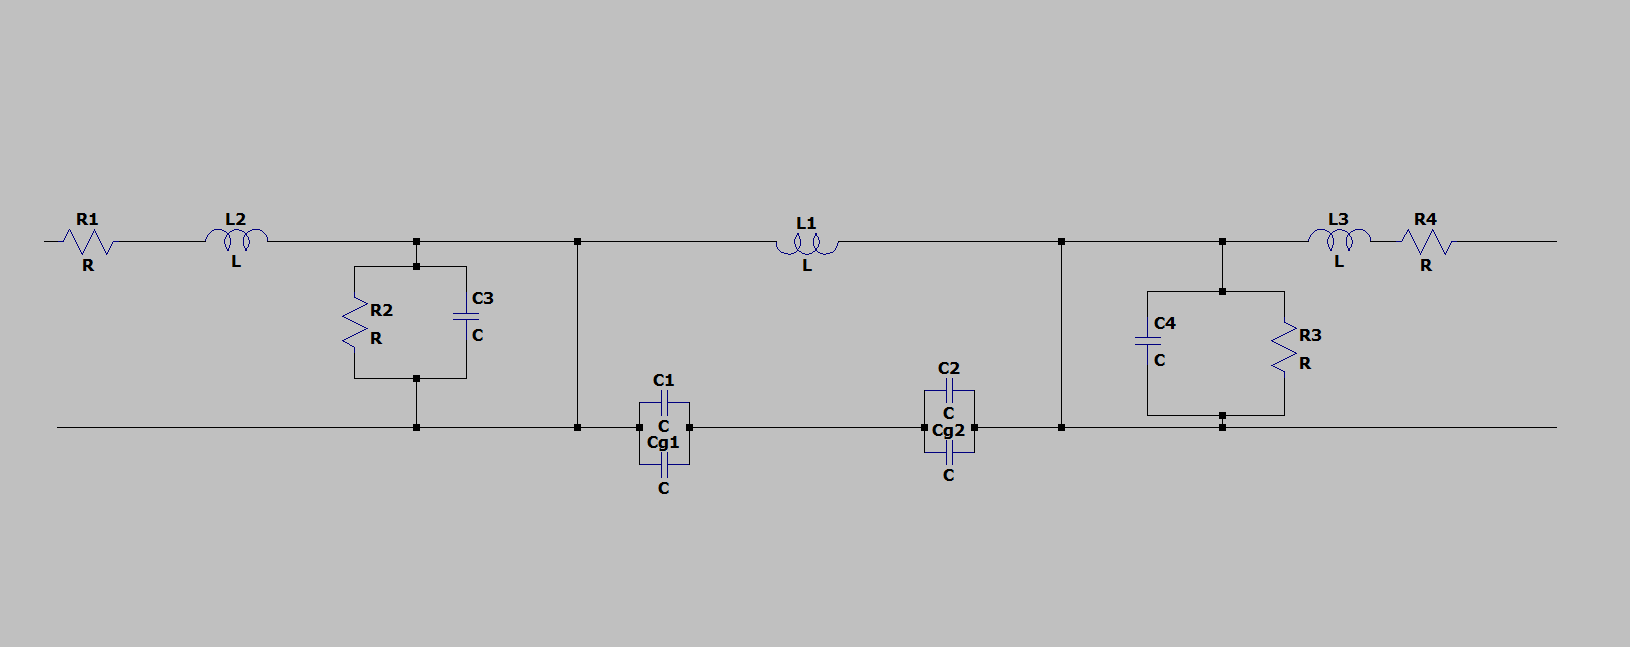
\includegraphics[width=0.25\textwidth]{Images/With_Transmission_line_Equivalent.png}
    \caption{Equivalent circuit model of a Double Ring SRR with Transmission Line.}
    % \label{fig:SRR_circuit}
\end{figure}


\begin{align}
    C_0 &= 2\pi r_0 C_{\text{pul}},  \\
    L_s &= \frac{4\pi^2 r_0^2 N^2}{1 + 0.45 \times 2 r_0},  \\
    C_c &= \frac{4 \varepsilon_0 L_s}{\mu_0},  \\
    L_0 &= \frac{C_0 \mu_0}{4 \varepsilon_0}. 
    \end{align}
    
    The resonant frequency of the fabricated CSRR can be expressed as Eq.~(5). By stretching the CSRR, an increase in \( r_0 \) causes an increase in capacitance and inductance, which ultimately causes a decrease in the resonant frequency,
    
    \begin{equation}
    f_p = \frac{1}{2\pi \sqrt{L_0 C_c}}. 
    \end{equation}

\begin{figure}[h]
\centering
    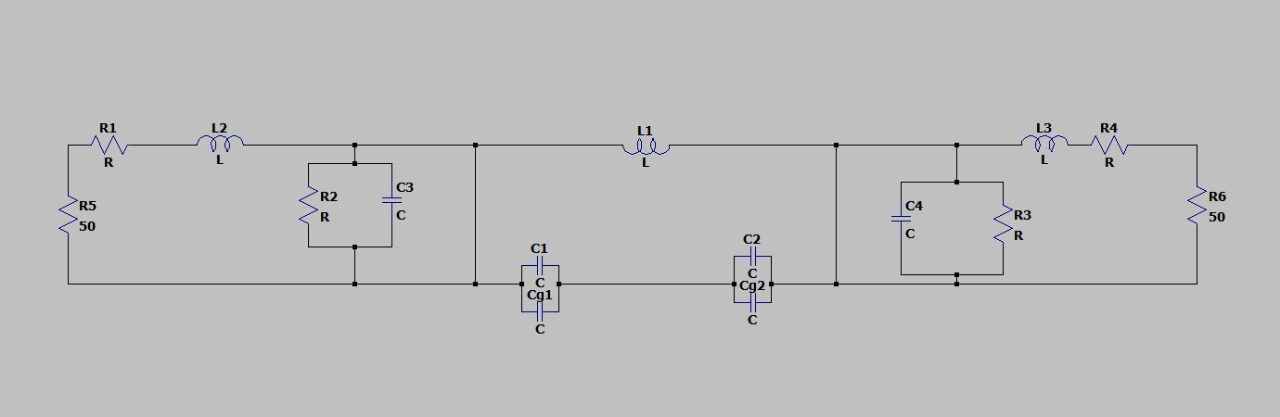
\includegraphics[width=0.5\textwidth]{Images/transmission_line_quarter_wave.jpg}
    \caption{Impedance matching using a quarter wave transformer.}
    % \label{fig:SRR_circuit}
\end{figure}

\subsection{Coupling Mechanisms}
Split Ring Resonators (SRRs) interact with electromagnetic fields primarily through two coupling mechanisms: magnetic (inductive) coupling and electric coupling. These mechanisms significantly influence their resonance behavior and are central to the design of metamaterials, filters, and sensors.

Magnetic coupling is driven by Faraday’s Law. A time-varying magnetic field from the current in one SRR induces an electromotive force (EMF) in a neighboring SRR, generating a circulating current. This mutual inductance leads to negative coupling, where the induced current opposes the original magnetic field (as per Lenz’s Law), causing the resonance frequencies to split or shift. Magnetic coupling is strongest when the SRRs are aligned with their loops facing the same direction but with gaps on opposite sides, maximizing magnetic flux linkage. This configuration is commonly used to achieve negative permeability and magnetic field confinement.

Electric coupling, on the other hand, occurs due to the interaction between the electric fields across the split gaps of SRRs. When the gaps are aligned or closely positioned, the electric field from one SRR induces a similar charge distribution across the gap of the neighboring SRR. This forms coupled electric dipoles that result in positive coupling. The fields reinforce one another, enhancing the overall electric field interaction and leading to upward resonance shifts. This effect is especially important in sensing applications, where field localization and sensitivity are crucial.

In practical configurations, both types of coupling can occur simultaneously. The relative orientation, gap alignment, and distance between SRRs can be strategically modified to fine-tune the overall coupling strength and resonance characteristics. This tunability is essential in designing components for metamaterials, reconfigurable filters, high-sensitivity sensors, and antennas.

\section{Design Methodology}

\subsection{Design Requirements and Specifications}
List the required performance: 5 GHz center, target bandwidth, notch depth, substrate limitations, and footprint constraints.

\subsection{Substrate Selection and Microstrip Design}
Describe chosen substrate (e.g., FR4 or Rogers), its dielectric constant, thickness, and loss tangent. Calculate 50-ohm microstrip width.

\subsection{SRR Topology Selection}
Compare various geometries (square, circular, spiral). Justify your selection based on performance and ease of fabrication.

\subsection{Parametric Analysis Framework}
Outline which parameters (gap, ring width, spacing) are to be swept in simulation. Describe your approach to optimization.

\subsection{Coupling Configuration}
Describe SRR placement relative to the microstrip. Provide geometry layout and explain expected coupling mode.

\subsection{Expected Performance}
Estimate resonant frequency using derived equations. Predict notch depth and bandwidth.

\section{Simulation Methodology}
The numerical method used in HFSS is the Finite Element Method (FEM). In this method a structure is subdivided into many small subsections called finite elements. In HFSS these finite elements are in the form of tetrahedra. The entire collection of tetrahedra constitutes the finite element mesh. A solution is found for the fields within these tetrahedra. These fields are
interrelated so that Maxwell’s Equations are satisfied across inter-element boundaries yielding a field solution for the entire original structure. Once the field solution is found, the generalized S matrix solution is determined.
The tool also uses the automatic adaptive mesh refinement process to solve an EM problem. To set up the design, we need to create the geometry and specify material properties, boundary conditions, excitations, and the solution frequency.


\subsection{HFSS Simulation Environment Setup}
Describe the overall simulation environment and settings.

\subsection{Material Properties and Model Creation}
Assign dielectric and conductor properties. Detail 3D model dimensions and layers in HFSS.

\subsection{Excitation and Boundary Conditions}
Explain port settings and boundary types (e.g., radiation boundary). Validate open-space behavior.

\subsection{Post-Processing Methods}
Outline how S-parameters, return loss, and electric/magnetic fields were extracted and visualized.

\section{Results and Analysis}
Final Double Ring SRR Design: 5 GHz Notch Filter
\begin{figure}[h]
\centering
    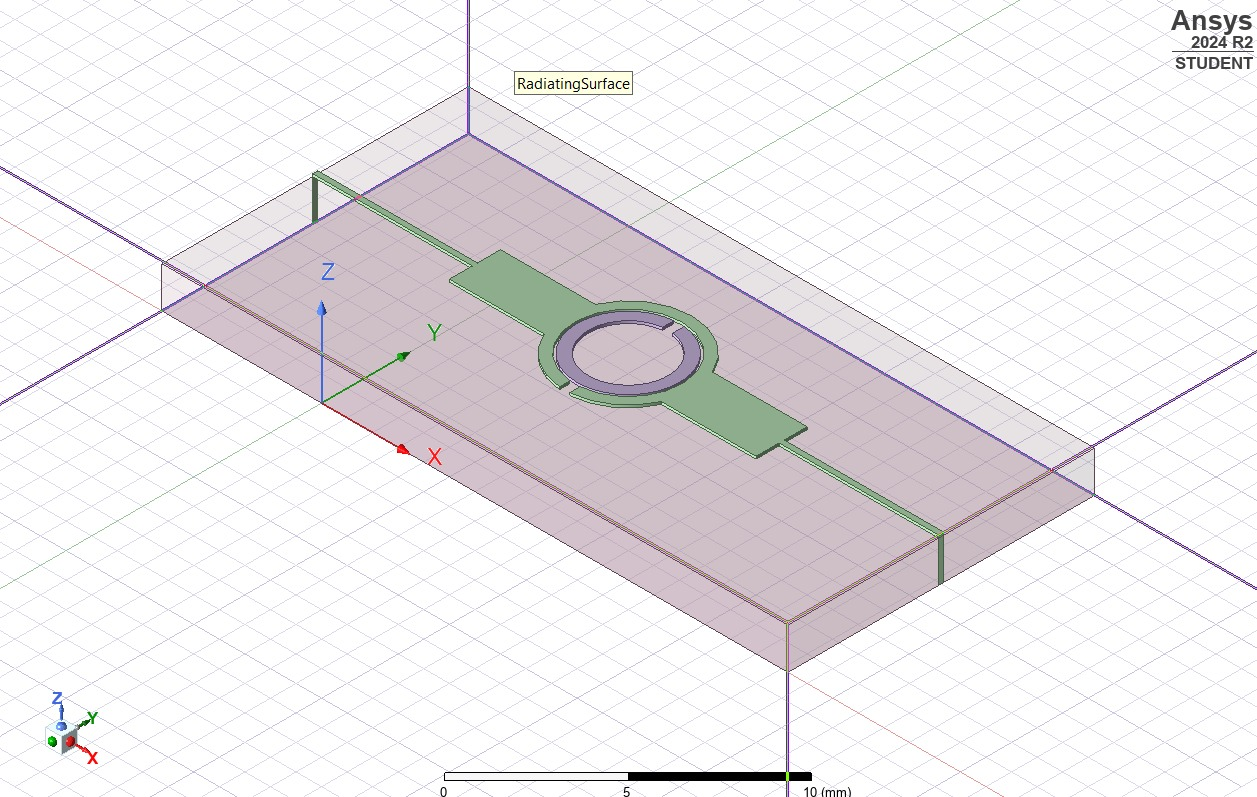
\includegraphics[width=0.5\textwidth]{Images/final_double_ring_srr.jpg}
    \caption{Final Double Ring SRR Design with Quarter Wave Transformer.}
    % \label{fig:SRR_circuit}
\end{figure}
\subsection{Resonance Frequency}

From the simulation results (S - Parameter plot), the resonant frequency is observed to be 4.96 GHz. The notch filter exhibits a sharp notch at this frequency, indicating effective filtering of signals around this frequency.

\subsection{Quality Factor}
The quality factor (Q-factor) is a measure of the sharpness of the resonance peak. It is defined as the ratio of the resonant frequency to the bandwidth of the filter. A higher Q-factor indicates a sharper resonance and better selectivity. The Q-factor can be calculated using the formula:
\begin{equation}        
    Q = \frac{f_o}{\Delta f}
\end{equation}
$Q = \frac{4.96}{5.05-4.8925} = \frac{4.96}{0.1575} = 31.49$

\subsection{Sensitivity}
Sensitivity is defined as the ratio of the change in resonant frequency to the change in the physical parameter (e.g., gap size, ring width). It can be calculated using the formula:
\begin{equation}        
    S = \frac{\Delta f}{\Delta X}
\end{equation}
where \( \Delta f \) is the change in resonant frequency and \( \Delta X \) is the change in the physical parameter.\\

$ S = \frac{4.96 - 4.6725}{2.6-1} = 0.1796$
\begin{figure}[h]
\centering
    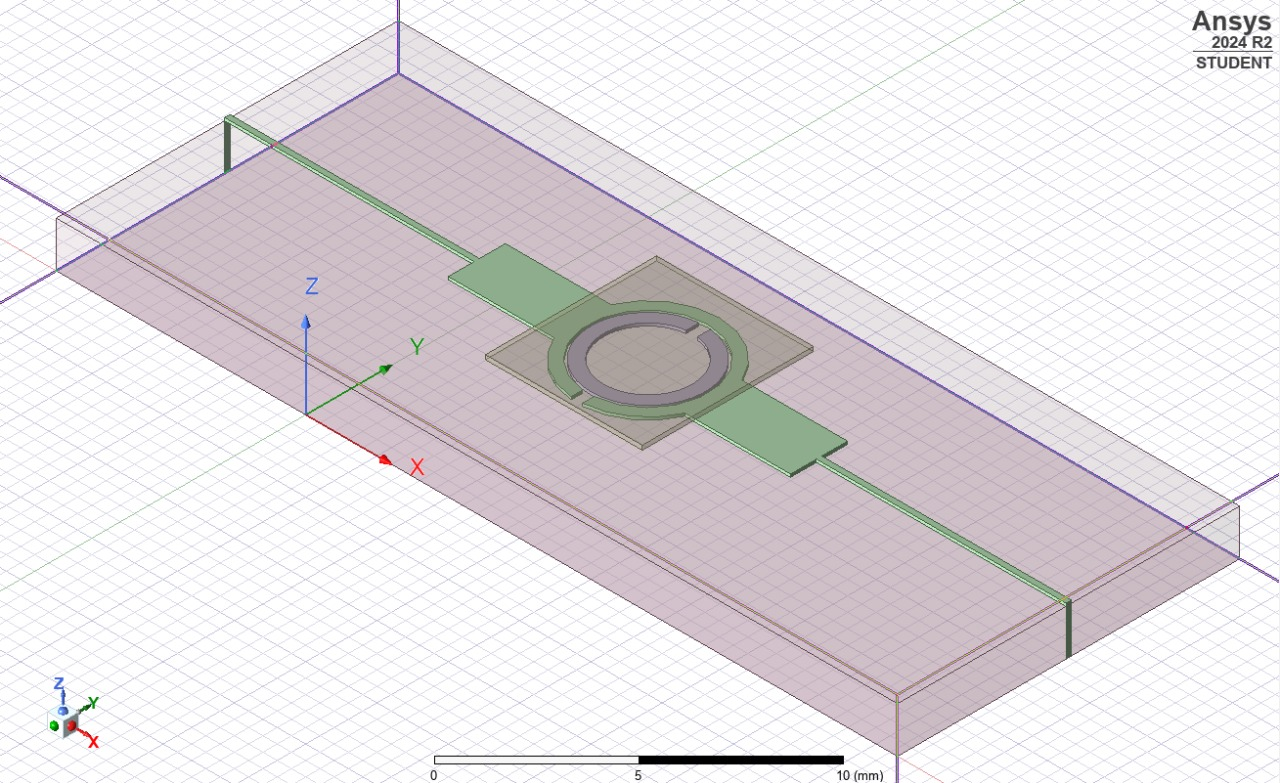
\includegraphics[width=0.5\textwidth]{Images/final_dielectric_sensitivity.jpg}
    \caption{SRR Notch filter with different analyte (Benzocyclobutene).}
    % \label{fig:SRR_circuit}
\end{figure}

\subsection{S-Parameter Results}
Final S-parameter results for the designed SRR notch filter are shown in the following figures. The S-parameters provide insight into the filter's performance, including return loss (S11) and insertion loss (S21).

We can clearly see that the S11 parameter is less than -10 dB at the notch frequency of 4.96 GHz, indicating a good return loss and effective filtering. The S21 parameter shows a significant drop at the notch frequency, confirming the filter's band-stop characteristics.

\begin{figure}[h]
\centering
    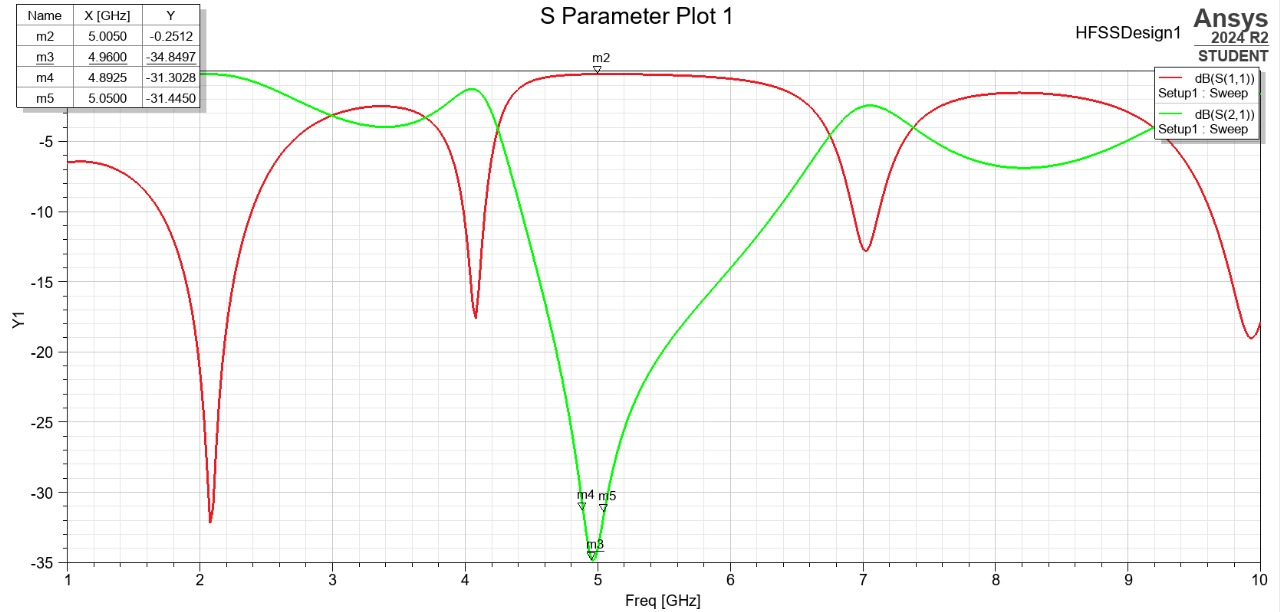
\includegraphics[width=0.5\textwidth]{Images/Fiinal_S_Param_Plot.jpg}
    \caption{S-parameter results for the designed SRR notch filter.}
    % \label{fig:SRR_circuit}
\end{figure}

\subsection{Z-Parameter Results}

Final Z-parameter results for the designed SRR notch filter are shown in the following figures. The Z-parameters provide insight into the filter's performance, including return loss (Z11) and insertion loss (Z21).

The marker m2 represents the impedance matching point, which is at 50 ohms. The Z11 parameter shows a good return loss at the notch frequency, indicating effective impedance matching. 

\begin{figure}[h]
\centering
    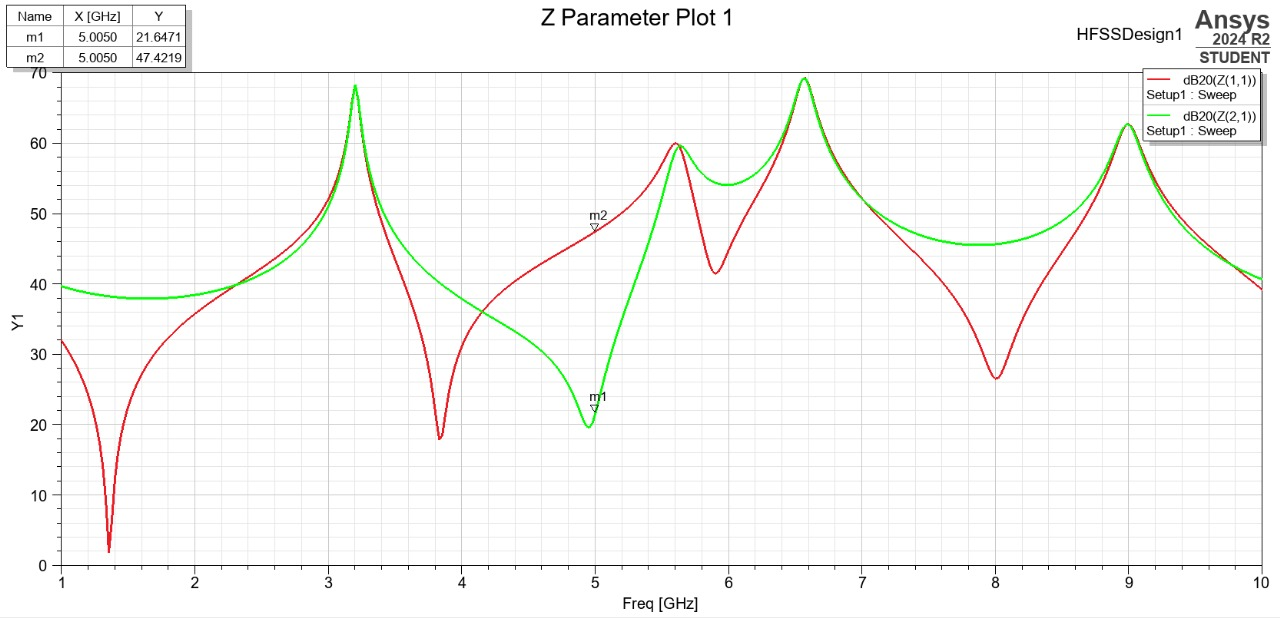
\includegraphics[width=0.5\textwidth]{Images/Final_Z_Param_Plot.jpg}
    \caption{Z-parameter results for the designed SRR notch filter.}
    % \label{fig:SRR_circuit}
\end{figure}

\section{Conclusion}
\subsection{Summary of Findings}
This work presents the design and simulation of a 5 GHz SRR notch filter using Ansys HFSS. The filter demonstrates a compact size, high selectivity, and effective notch characteristics. The use of a double-ring circular SRR enables miniaturization, resulting in a compact filter layout suitable for modern RF front-end applications.

\subsection{Significance of the Results}
The designed SRR notch filter is a planar structure that can be easily integrated into existing RF systems. The sharp notch and strong rejection provide excellent interference mitigation for targeted frequency bands. 

\subsection{Limitations and Future Work}
The current SRR-based notch filter design has limitations, including a fixed notch frequency without tunability, reliance on idealized simulations that do not account for real-world factors like fabrication tolerances and substrate losses, and the absence of experimental validation. Future work could focus on integrating varactors or PIN diodes to enable tunable or switchable rejection, developing multi-band configurations by combining multiple SRRs, coupling the filter with wideband antennas for system-level analysis, and exploring advanced substrates to enhance miniaturization and performance.


\begin{thebibliography}{00}
\bibitem{b1} S. Dasi, S. Dasi and G. M. Rao, "Design and Analysis of a Meta Material based Nested Circular Split Ring Resonator for Terahertz Applications," 2022 International Conference on Automation, Computing and Renewable Systems (ICACRS), Pudukkottai, India, 2022, pp. 178-181, doi: 10.1109/ICACRS55517.2022.10029069.

\bibitem{b2}C. Saha and J. Y. Siddiqui, "A comparative analyis for split ring resonators of different geometrical shapes," 2011 IEEE Applied Electromagnetics Conference (AEMC), Kolkata, India, 2011, pp. 1-4, doi: 10.1109/AEMC.2011.6256871.

\bibitem{b3}

\bibitem{b4}

\bibitem{b5}

\bibitem{b6}

\bibitem{b7}

\bibitem{b8}

\bibitem{b9}

\bibitem{b10}

\end{thebibliography}

\end{document}
